
\section{Zielsetzung}
Das Ziel des Versuchs ist es Leerlaufspannung und Innenwiderstände von verschiedenen
Spannungsquellen zu messen.

\section{Theorie}
Eine Spannungquelle ist ein Gerät, welches über einen langen Zeitraum konstante Leistung liefert.
In Abbildung \ref{fig:messung1} ist das Schaltbild einer realen Spannungsquelle gestrichelt
dargestellt, welche aus einem Innenwiderstand $R\ua{i}$ besteht, der mit der Sapnnungsquelle in
Reihe geschaltet ist.
Als Leerlaufspannung $U\ua{0}$ wird die Spannung bezeichnet, die an den Ausgangsklemmen
gemessen wird, wenn die Innenwierstände $R\ua{i} = 0$ sind.
\newline
Fließt über einen äußeren Lastwiderstand $R\ua{a}$ ein endlicher Strom $I$ wird die sogenannte
Klemmspannung $U\ua{k}$ gemessen.
Mit dem zweiten Kirchhoffschen Gesetz
\begin{align}
  \sum\ua{i}U\ua{i} &= 0
\end{align}
sowie mit dem Ohmschen Gesetz $U =R \cdot I$ folgt für die Leerlaufspannung
\begin{align}
  U\ua{0} &= I(R\ua{i} + R\ua{a})
\end{align}
und somit für die Klemmspannung
\begin{align}
   U\ua{k} &= IR\ua{a} = U\ua{0} - IR\ua{i}.
\end{align}
Für die Messung der Leerlaufspannung wird ein hochohmiges Voltmeter verwendet, weshalb
der fließende Strom gering ist. Deshalb gilt für die Leerlaufspannung $U\ua{k} ≈ U\ua{0}$.
\newline
Die Innenwiderstände beschränken die Leistung der Spannungsquelle. Durch
\begin{align}
  N &= I^{2}R\ua{a} = N(R\ua{a})
\end{align}
wird die abgegeben Leistung an den Lastwiderstand $R\ua{a}$ beschrieben. Für $R\ua{a} = R\ua{i}$
wird $R\ua{a}$ so angepasst, dass die Leistung $N$ maximal ist.
\newline
Bei elektrische Generatoren ist der Innenwiderstand durch Rückkopplungsmechanismen festgelegt.
Somit bestimmen Änderungen des Belastungsstromes das elektrische Verhalten der Spannungsquelle.
In diesem Fall muss der Innenwiderstand als differtielle Größe betrachtet werden:
\begin{align}
  R\ua{i} &= \frac{dU\ua{k}}{dI}
\end{align}
\newpage
\section{Aufbau und Durchführung}
Im ersten Teil des Versuchs wird die Leerlaufspannung einer Monozelle mit ihrem zugehörigen
Eingangswiderstand $R\ua{v}$ an einer Schaltung wie in Abbildung \ref{fig:messung1} bestimmt.
\begin{figure}[H]
  \centering
  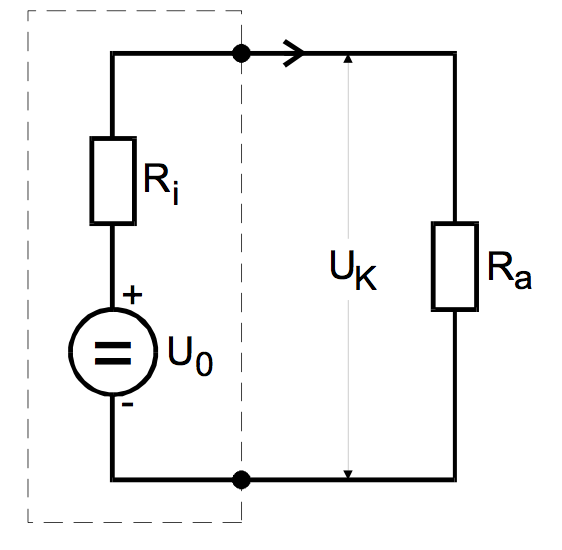
\includegraphics[scale = 0.7]{aufbau1.PNG}
  \caption{Schaltbild einer realen Spannungsquelle}
  \label{fig:messung1}
\end{figure}

Im zweiten Teil des Versuchs wird der Schaltkreis wie in Abbildung \ref{fig:messung2} mit einem Amperemeter
und einem regelbaren Widerstand erweitert. Hierbei kann der Widerstand zwischen $0-50\su{\Omega}$
variiert werden. In Abhängigkeit des Belatungsstroms $I$ wird die Klemmspannung $U\ua{k}$ gemessen.
\begin{figure}[H]
  \centering
  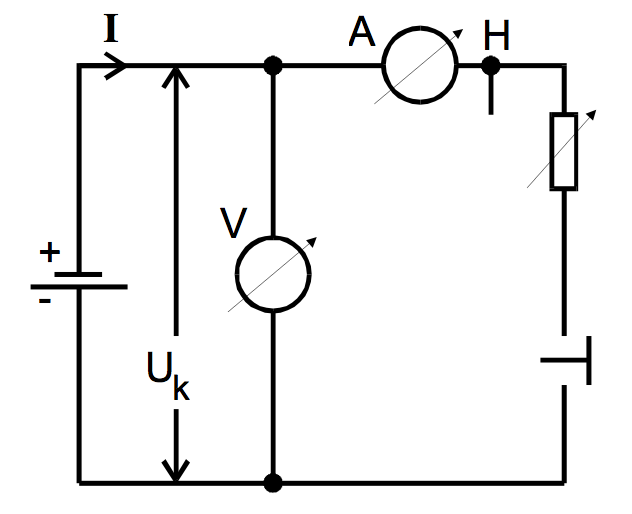
\includegraphics[scale = 0.7]{aufbau2.PNG}
  \caption{Schaltung zur Bestimmung der Klemmspannung}
  \label{fig:messung2}
\end{figure}

Durch die Erweiterung mit einer in Reihe geschalteten Gegenspannung, wie in Abbildung \ref{fig:messung3}
zu sehen ist, wird erneut die Klemmspannung $U\ua{k}$ in Abhängigkeit des Stromes $I$ bestimmt.
Der Strom fließt nun in die entgegensetzte Richtung. Daraus folgt für die Klemmspannung
\begin{align}
U\ua{k} &= U\ua{0} +IR\ua{i}.
\end{align}

\begin{figure}[H]
  \centering
  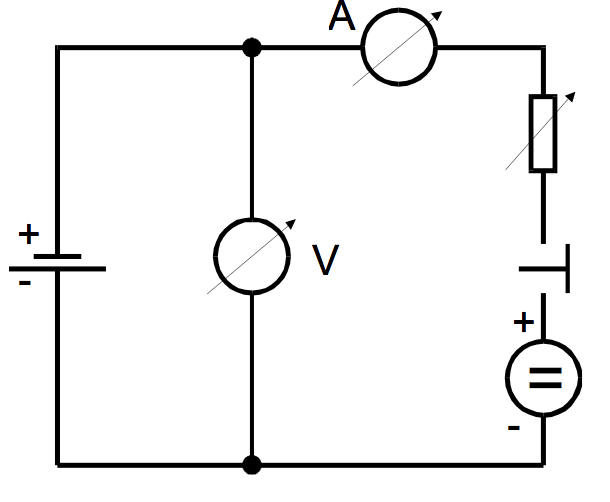
\includegraphics[scale = 0.7]{aufbau3.PNG}
  \caption{Schaltung mit Gegenspanung}
  \label{fig:messung3}
\end{figure}

Die Abbildung \ref{fig:messung1} wird anschließend für erneute Messung von $U\ua{k}$ verwendet. Als Messobjekt
werden eine Sinus- und Rechteckspannung angelegt. Der regelbare Widerstand beträgt dabei für
die Sinuspannung $0.1-5\,\mathrm{k\Omega}$ und für die Rechteckspannung $20-250\su{\Omega}$.
%bei 0.1-5 muss es kiloohm sein! wie geht das?
